\documentclass{beamer}

% Romanian Language support
\usepackage{ucs}
\usepackage[utf8x]{inputenc}
\PrerenderUnicode{aâîțșĂÎÂȚȘ}
\usepackage[english,romanian]{babel}

\usepackage{hyperref}   % use \url{http://$URL} or \href{http://$URL}{Name}
\usepackage{verbatim}
\usepackage{underscore} % underscores need not be escaped
\usepackage{booktabs}   % nice looking tables
\usepackage{array}      % column size options in tables
\usepackage[normalem]{ulem}       % for striketrough text

\mode<presentation>
%{ \usetheme{Berlin} }

% Disable useless navigation symbols.
\setbeamertemplate{navigation symbols}{}

\title[Cuvintele au putere]{Cuvintele au putere}
\institute{InfoEducație 2017 (Gălăciuc, Vrancea)}
\author[Răzvan Deaconescu]{Răzvan Deaconescu \\
razvan.deaconescu@cs.pub.ro}
\date{3 august 2017}

\begin{document}

\frame{\titlepage}

\begin{frame}{Să vedem și să ascultăm}
  \begin{center}
    \scriptsize
    \url{link la World of Warcraft: Wrath of the Lich King intro}
  \end{center}
\end{frame}

\begin{frame}{Napoleon dixit}
  \centering
  \textit{A man does not have himself killed for a half-pence a day or for a petty distinction; you must speak to the soul in order to electrify him.}\\
  \vspace{3mm}
  \hfill \textit{Napoleon Bonaparte}
\end{frame}

\begin{frame}{Să vedem și să ascultăm}
  \begin{center}
    \scriptsize
    \url{link la discursul lui V}
  \end{center}
\end{frame}

\begin{frame}{Esop dixit}
  povestea cu limbile
\end{frame}

\begin{frame}{Cuvinte}
  gri vs. sur vs. cenușiu \\
  \begin{figure}
    \centering
    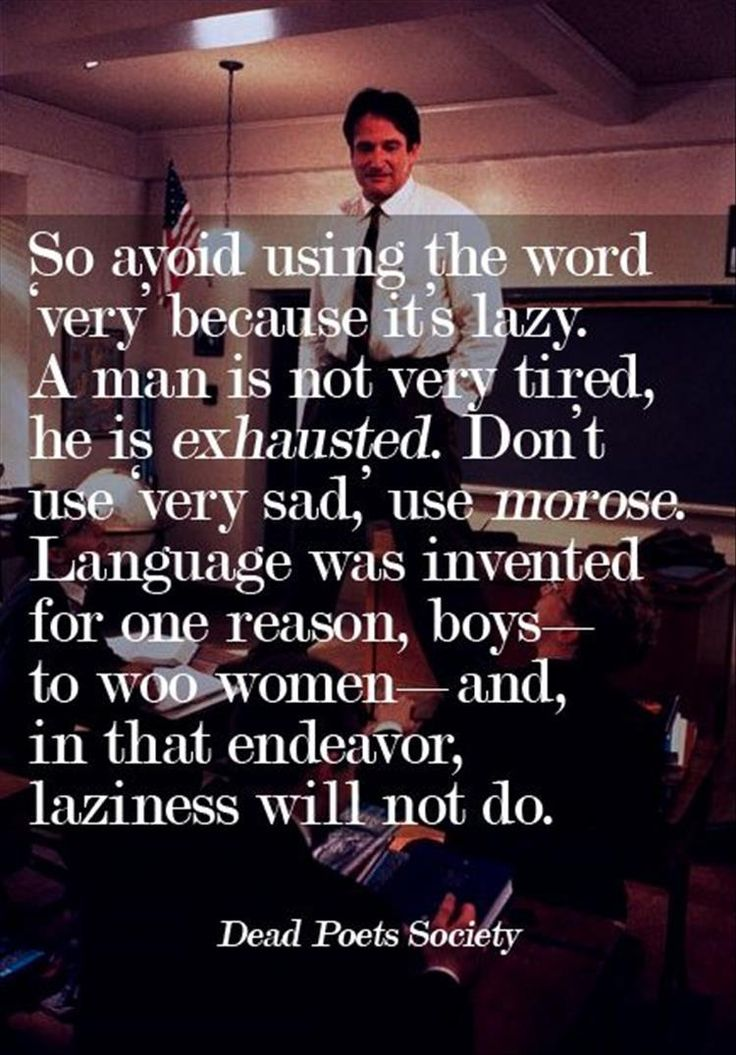
\includegraphics[width=0.4\textwidth]{img/dead-poets-society-lazy}
  \end{figure}
  \begin{center}
    \tiny
    \url{https://s-media-cache-ak0.pinimg.com/736x/6c/54/e6/6c54e6b4cd05585523d3ce5ae5a55574--robin-williams-writing-tips.jpg}
  \end{center}
\end{frame}

\begin{frame}{Unde folosim cuvinte?}
  conversatii, informatii, articole, esee
  citate, literatura, discursuri, dezbateri
\end{frame}

\begin{frame}{Cuvant scris, cuvant vorbit}
  scriere vs. vorbire
  mai multa putere are cel vorbit
  de ce exista cuvant scris
  citit scris de cineva, ascultat ce zice cineva, urmarit cand cineva zice
\end{frame}

\begin{frame}{Tipuri de limbaj}
  verbal, non-verbal, para-verbal
  discard what you hear in favor of what you see
\end{frame}

\begin{frame}{Ca sa-l citam pe Barack Obama}
  ,,You know I've got to talk about Donald Trump, right?''
  8\% fapte, dar prinde
  nepregatit, neinformat, fara viziune, fara o pozitie politica consecventa, dar prinde
  cuvinte simple
  agresivitate si dominanta
  set the agenda
  lucreaza pe psihic/emotie (4D chess: Scott Adams)
  \begin{figure}
    \centering
    
\includegraphics[width=0.4\textwidth]{img/love-trumps-hate}
  \end{figure}
  \begin{center}
    \tiny
    \url{http://www.imediaethics.org/wp-content/uploads/2015/12/lovetrumpshate.jpg}
  \end{center}
\end{frame}

\begin{frame}{Controlul conversatiei: rolul cuvintelor}
  \begin{center}
    \scriptsize
    \url{link la interviu cu sustinator Hillary Clinton}
  \end{center}
  \centering
  \textit{Fere libenter homines id quod volunt credunt.}
  \vspace{3mm}
  \hfill \textit{Gaius Julius Caesar}
  argumentele factuale pot fi folosite doar in anumite situatii
  in mai multe situatii merg exprimari de control psihologic/emotional
\end{frame}

\begin{frame}{Ronald Reagan: The Great Communicator}
  \begin{center}
    \scriptsize
    \url{link la replică legată de vârstă}\\
    \url{la replică yes, I was a democrat}
  \end{center}
\end{frame}

\begin{frame}{Reframing}
  \begin{center}
    \scriptsize
    \url{Tyrion Lannister vs. Shagga}\\
    \url{Rob Stark vs. Jaime Lannister}
  \end{center}
\end{frame}

\begin{frame}{What happened here?}
  \begin{center}
    \scriptsize
    \url{Tyrion Lannister vs. Daenerys Targaryen}
  \end{center}
  flipping the script
\end{frame}

\begin{frame}{Agree and amplify}
  esti cam ipocrit
  esti cam scund
  esti cam copilaros
  vorbesti cam repede
\end{frame}

\begin{frame}{Defectele ca armura}
  \centering
  \textit{Let me give you some advice bastard. Never forget what you are. The rest of the world will not. Wear it like armor, and it can never be used to hurt you.}\\
  \vspace{3mm}
  \hfill \textit{Tyrion Lannister (to Jon Snow)}
\end{frame}

\begin{frame}{Body Language}
  limbajul non-verbal
  corelat cu mindset-ul
  "te miroase"
\end{frame}

\begin{frame}{Cum ajungi la public/interlocutor?}
  creare (cuvinte) vs livrare (discurs)
  public, mindset
  \centering
  \textit{Un discurs este o discuție cu cineva, în care acel cineva este foarte important.}
  \vspace{3mm}
  \hfill \textit{Andrei Pleșu}
  keep it simple
  autenticitate / convergenta: fake it until you make it
  perceptie
  emotie vs. informatie: reminder citat din Napoleon, docere, movere, delectare
\end{frame}

\begin{frame}{Cum nu ajungi la public?}
  \centering
  \textit{TODO: Sorin Eftene}
  \begin{figure}
    \centering
    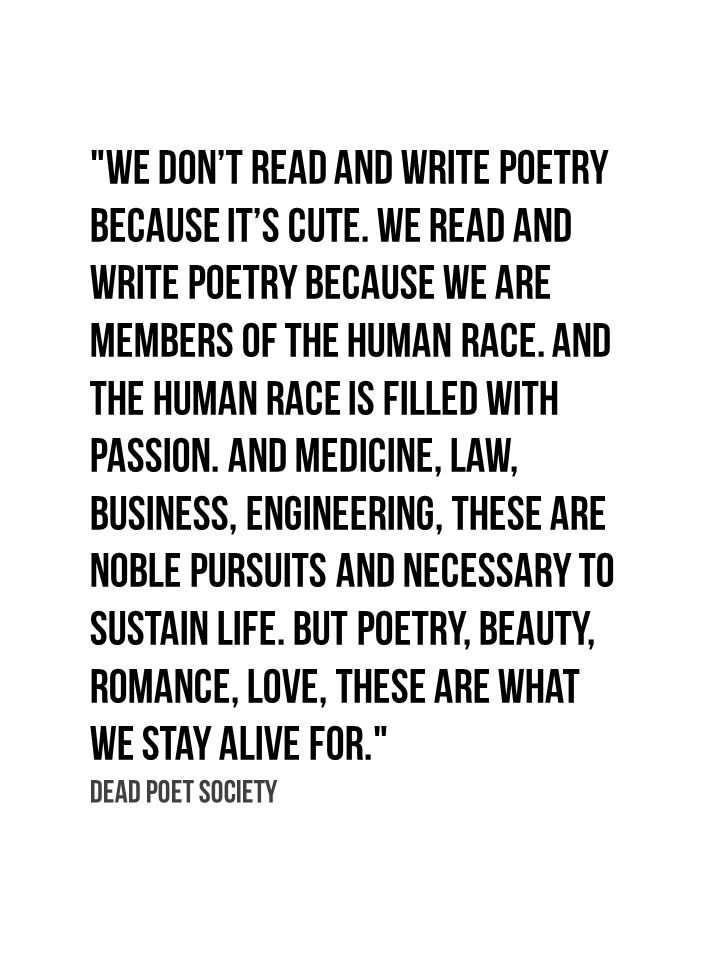
\includegraphics[width=0.4\textwidth]{img/dead-poets-society-words-alive} % TODO: Spiru Haret
  \end{figure}
\end{frame}

\begin{frame}{Spusul de povești / Storytelling}
  ce urmaresti in story telling?
  demo
  \centering
  \textit{Mâna întinsă care nu spune o poveste, nu primește pomană.}
  \vspace{3mm}
  \hfill \textit{Pavel Puiuț (Filantropica, 2002)}
\end{frame}

\begin{frame}{Cuvinte, poezie, emoție}
  \begin{figure}
    \centering
    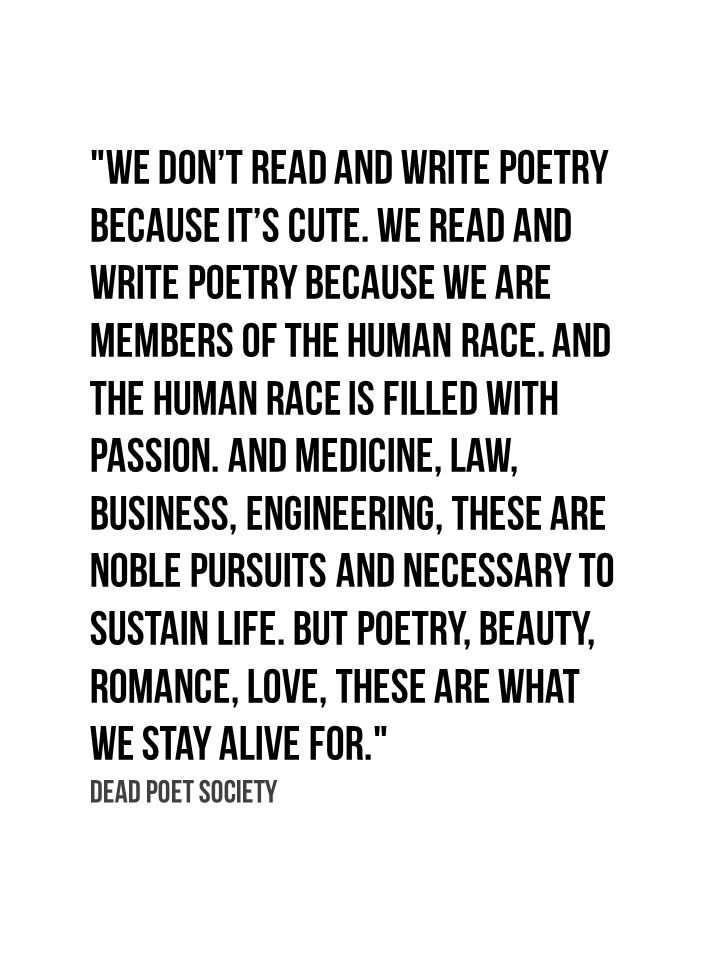
\includegraphics[width=0.4\textwidth]{img/dead-poets-society-words-alive}
  \end{figure}
  \begin{center}
    \tiny
    \url{https://s-media-cache-ak0.pinimg.com/736x/a6/2d/85/a62d85757ae9854952281e9375314115--dead-poets-society-quotes-favorite-movie-quotes.jpg}
  \end{center}
\end{frame}

\begin{frame}{Vorbit bine}
mapa, logare, caracter, creere, sa creem, librarie, a compresa
the right words
the right tone
the right posture
the right frame: mindset, storytelling, convergenta
\end{frame}

\begin{frame}{Cum ajungi la vorbit bine}
  citit, citit, citit
  \centering
  \textit{My mind is my weapon. My brother has his sword, King Robert has his warhammer and I have my mind\ldots{} and a mind needs books as a sword needs a whetstone if it is to keep its edge. That's why I read so much, Jon Snow.}\\
  \vspace{3mm}
  \hfill \textit{Tyrion Lannister (to Jon Snow)}
  experiență, vine cu vârsta, poate fi accelerată
  stat în lumina reflectoarelor
  dezbătut pe orice subiect
  scris esee, blog-uri
  citit și spus povești
  urmărit filme: dialog și poveste (scenariu)
  jocuri: dialog, poveste
  urmărit stand-up-uri
  trolling
  observat
  \centering
  \textit{It usually takes me more than three weeks to prepare a good impromptu speech.}
  \vspace{3mm}
  \hfill \textit{Mark Twain}
  corectat
\end{frame}

\begin{frame}{Făcut mișto-uri}
  defecte ca armură
  Joffrey Baratheon: \textit{If I tell the Hound to cut you in half, he'll do it without a second thought.}\\
  Tyrion Lannister: \textit{That would make me the quarter-man. Just doesn't have the same ring to it.}\\
  ball busting
  detașare, dispassionate, ZFG
  să poți face mișto de orice credință (nu vei pierde controlul)
  călire
\end{frame}

\begin{frame}{De ce asta?}
  cuvintele sunt parte din modul în care merge lumea
  job-urile viitorului (multă automatizare)
  persuasiune/negociere/manipulare
  crearea și menținerea de relații
  giving back/mentoring/passing knowledge
  popularitate/apreciere/autoritate
  înțelegerea mesajului și subtilităților, înțelegerea succesului
\end{frame}

\begin{frame}{Cuvintele au putere}
  \begin{figure}
    \centering
    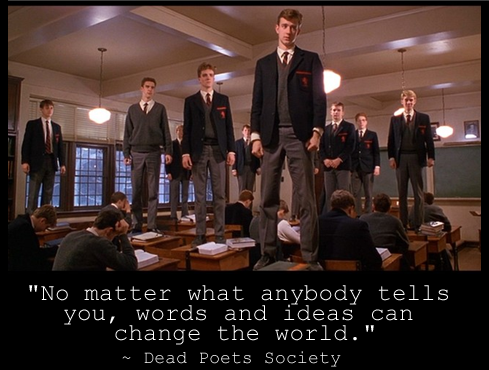
\includegraphics[width=0.4\textwidth]{img/dead-poets-society-words-change}
  \end{figure}
  \begin{center}
    \tiny
    \url{https://s-media-cache-ak0.pinimg.com/736x/43/ed/d5/43edd52f6d3b0c51925ff2fadd7e369e--peter-weir-peter-otoole.jpg}
  \end{center}
\end{frame}

\end{document}
